To find the table and balls it is important to understand how the table and balls appear in different color spaces. In this section the colors of the table and the pool balls will be measured for further analysis.\\

\subsubsection{The table}
As written in the rules\ref{sec:rules} the table cloth colour has to be yellow-green, blue-green or electric blue. The cloth color should be constant, but dependent on the lightning the variance of the cloth on the input image could be significant.

The table which has been used for measuring is a pool table with blue-green cloth which is located in Aalborg University's lab at Niels Jernes Vej 12 in room A6-314.

Three different images of the pool table and one image with the cloth cut out are analysed first in HSV color space and then i RGB space. These analysis will be used in the solution chapter.

\begin{figure}[H]
\begin{center}
\leavevmode
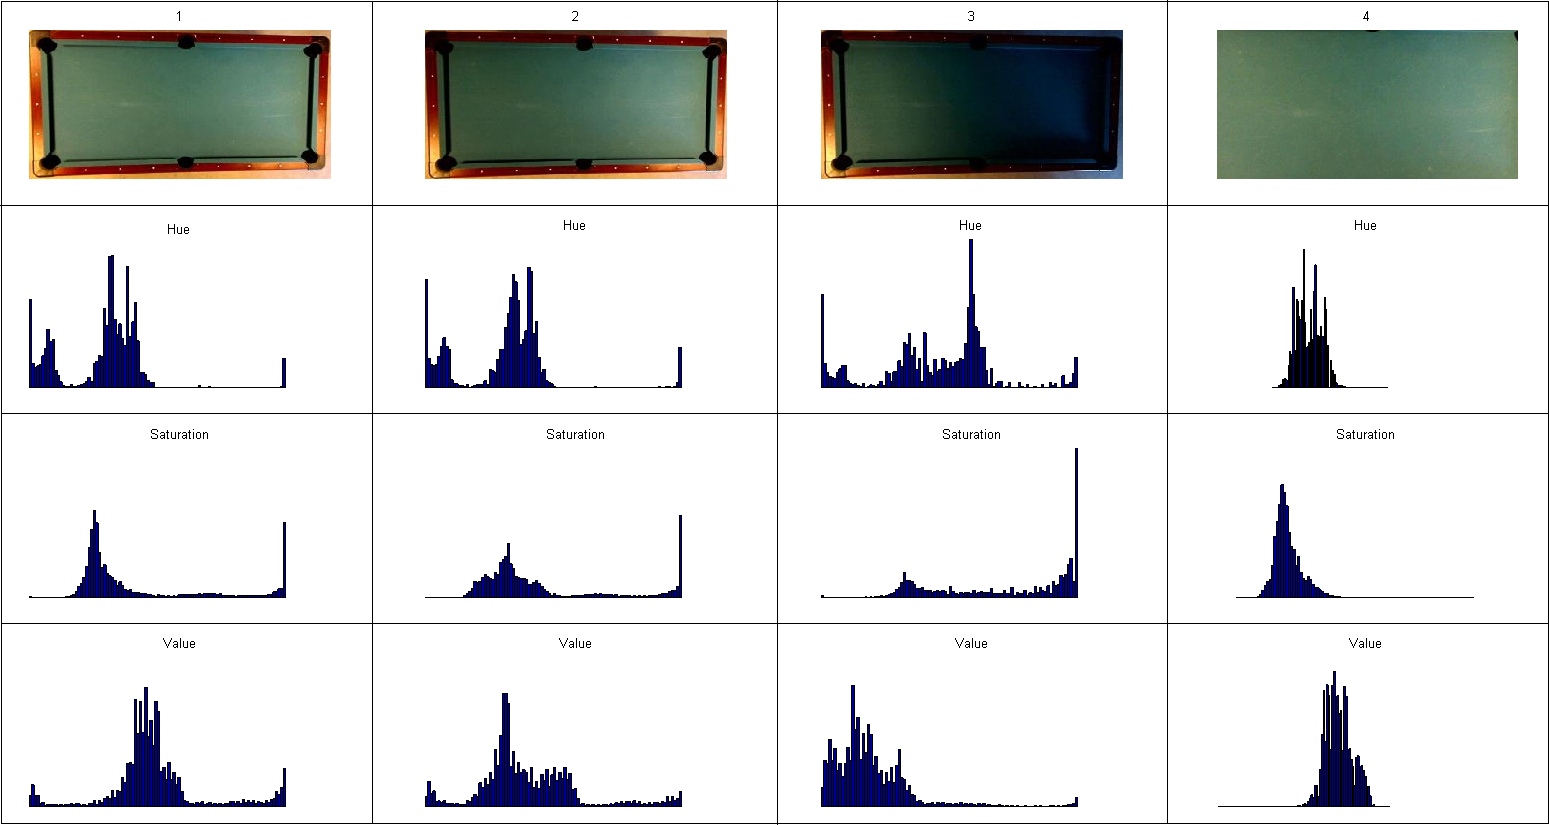
\includegraphics[width=1\textwidth]{images/hsv_hist_table}
\end{center}
\caption{HSV Images 1, 2 and 3 are mixed lightning where 4 is the cutout of the cloth from image 1. All axis are aligned.}
\label{fig:tablehsv}
\end{figure}

\begin{figure}[H]
\begin{center}
\leavevmode
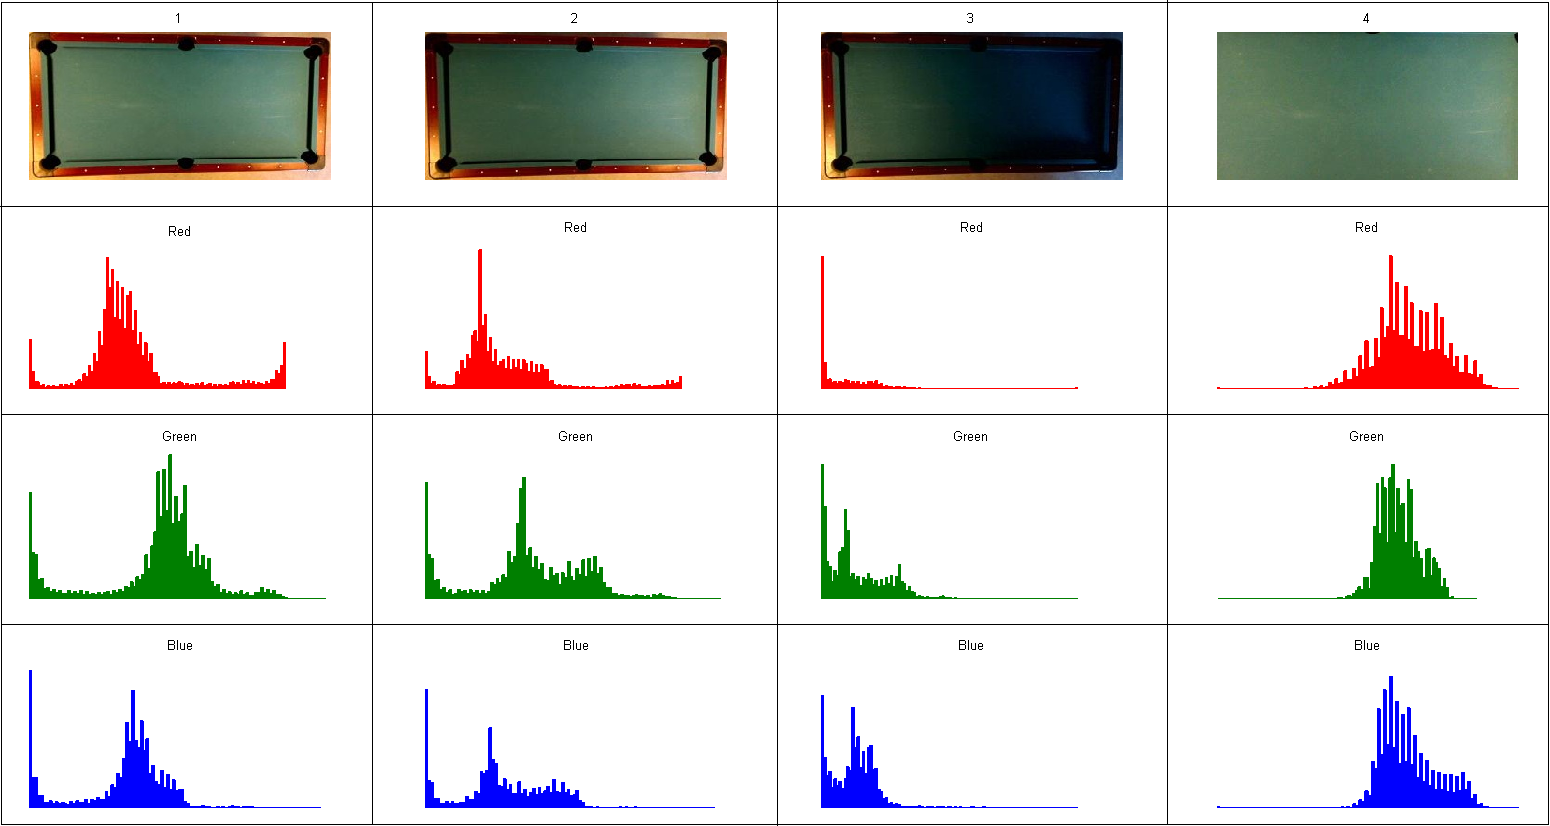
\includegraphics[width=1\textwidth]{images/rgb_hist_table}
\end{center}
\caption{RGB Images 1, 2 and 3 are mixed lightning where 4 is the cutout of the cloth from image 1. All axis are aligned.}
\label{fig:tablergb}
\end{figure}

From the HSV color space figure in \ref{fig:tablehsv} it is clear that the cloth should be somewhat easily found using hue for the fist two images. The separation of rail and cloth is not as significant in the third image. This is because of the different illumination, which is very dark. In section \ref{sec:camera} different camera settings and illuminations are discussed which indicates that the third image is less illuminated than should be for this project.\\

When looking at the RGB color space in figure \ref{fig:tablergb} the identification of the cloth becomes more difficult. As presumed the change in the RGB color space would be more significant for the cloth (fourth image) than the other images compared to the HSV color space \ref{fig:tablehsv}. This is because of the hue ability to be, in theory, illumination invariant.\\

\subsubsection{The balls}
\label{sec:analballs}
The success of the system depends on the identifier to be able to separate the pool balls from each other. To analyze the separability, histograms of all the different solid colored balls has been computed. This has been done in hue-saturation space, to see if it is possible to be independent of brightness. If the system is independent of brightness, it will be more resistant towards changes in light. The histograms are arranged pairwise together in the same figure, based on color similarity, to visualize how the colors can be separated.

\begin{figure}[H]
\centering
\subfloat
{
	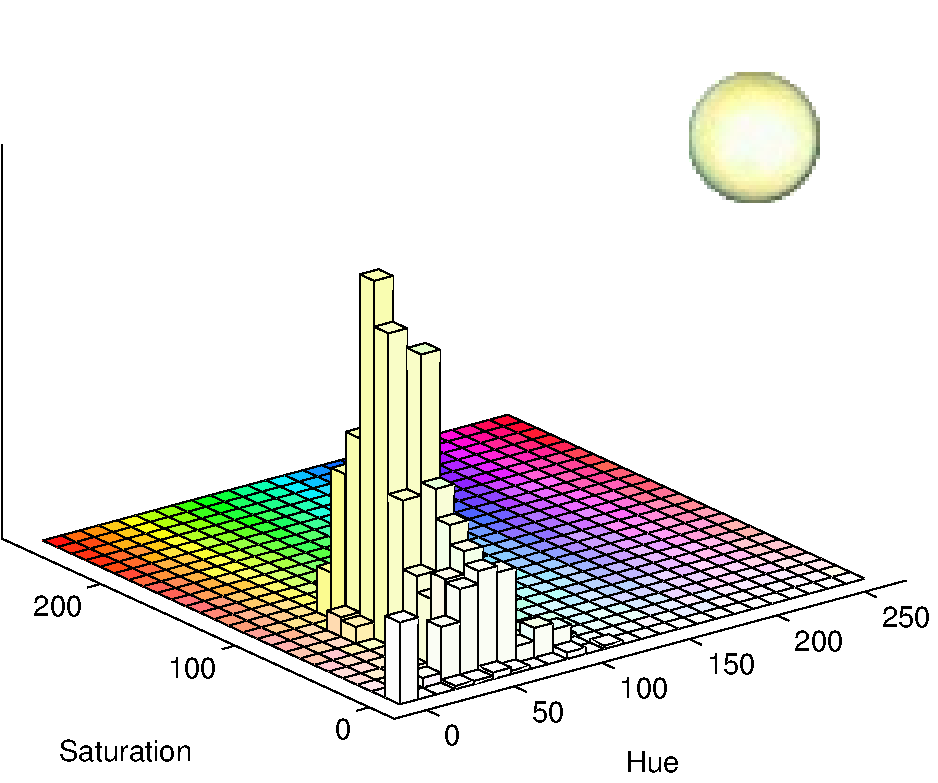
\includegraphics[width=0.4\textwidth]{images/ballhist/0}
}
\subfloat
{
	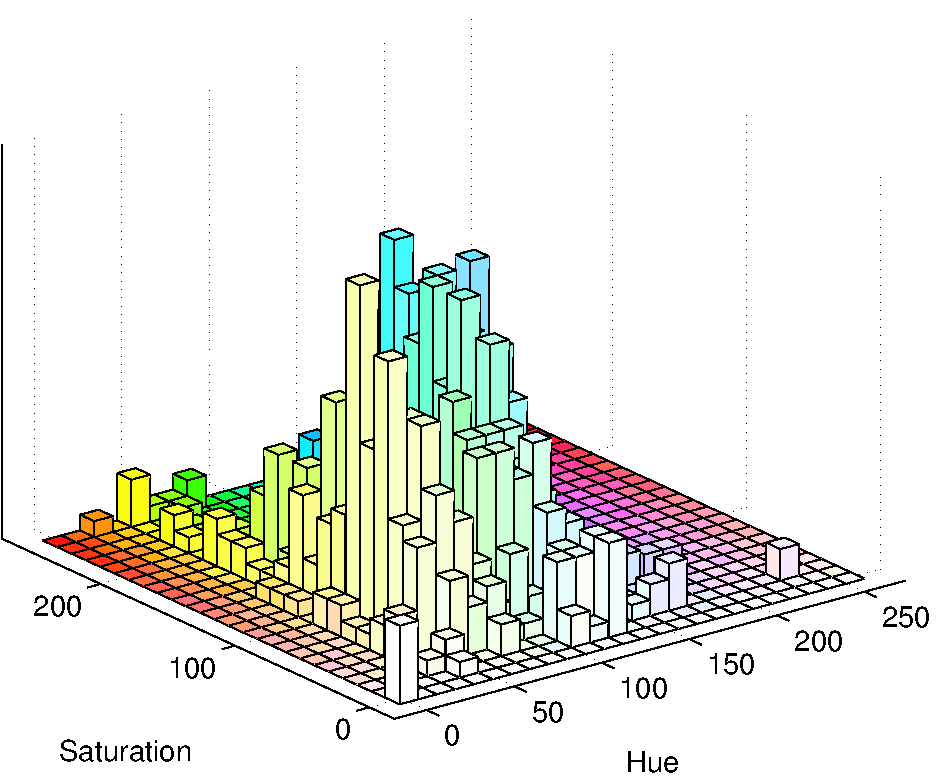
\includegraphics[width=0.4\textwidth]{images/ballhist/8}
}
\caption{Color histogram of cue-ball and 8-ball}
\label{fig:ballhist-cue-8}
\end{figure}
Figure \ref{fig:ballhist-cue-8} shows the histograms of the cue-ball and the 8-ball. The cue-ball distribution is isolated in a low-saturation area, having a yellow hue around 50. The saturation of the other balls is generally above the white saturation, making it possible to identify white pixels by setting a saturation threshold.

The hue-saturation distribution of the 8-ball is scattered all over the range. The reason for this, is that black is undefined in hue-saturation space. Black will have to be detected by the brightness value, which is significantly lower than other balls. \fxnote{VALUE HISTOGRAM HERE.}

\begin{figure}[H]
\centering
\subfloat
{
	
\includegraphics[width=0.4\textwidth]{images/ballhist/3}
}
\subfloat
{
	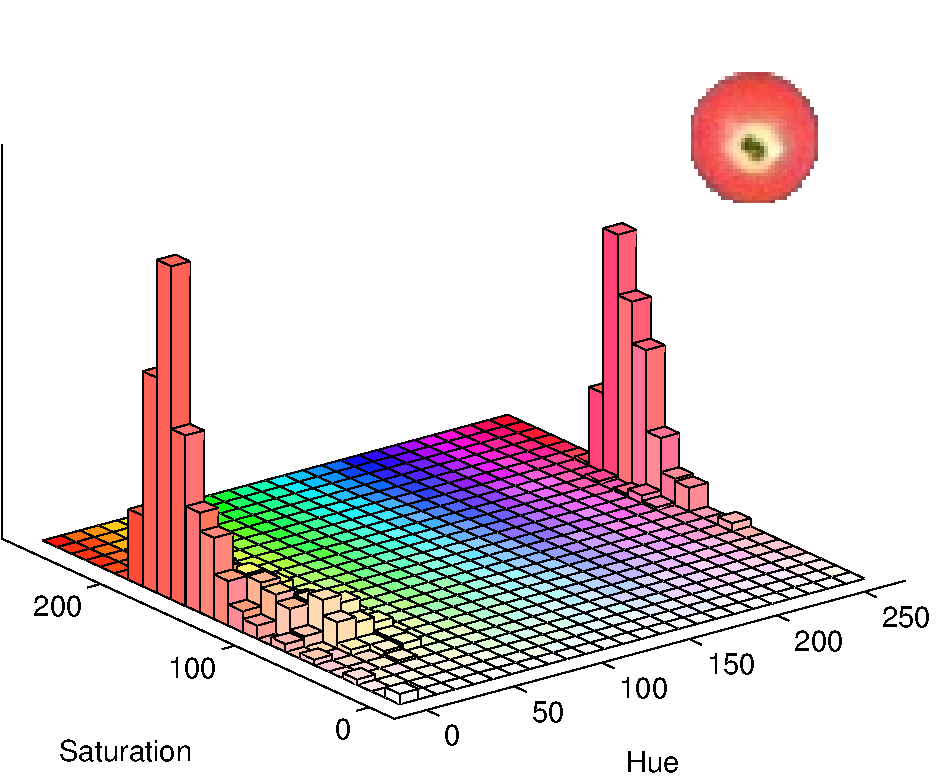
\includegraphics[width=0.4\textwidth]{images/ballhist/5}
}

\subfloat
{
	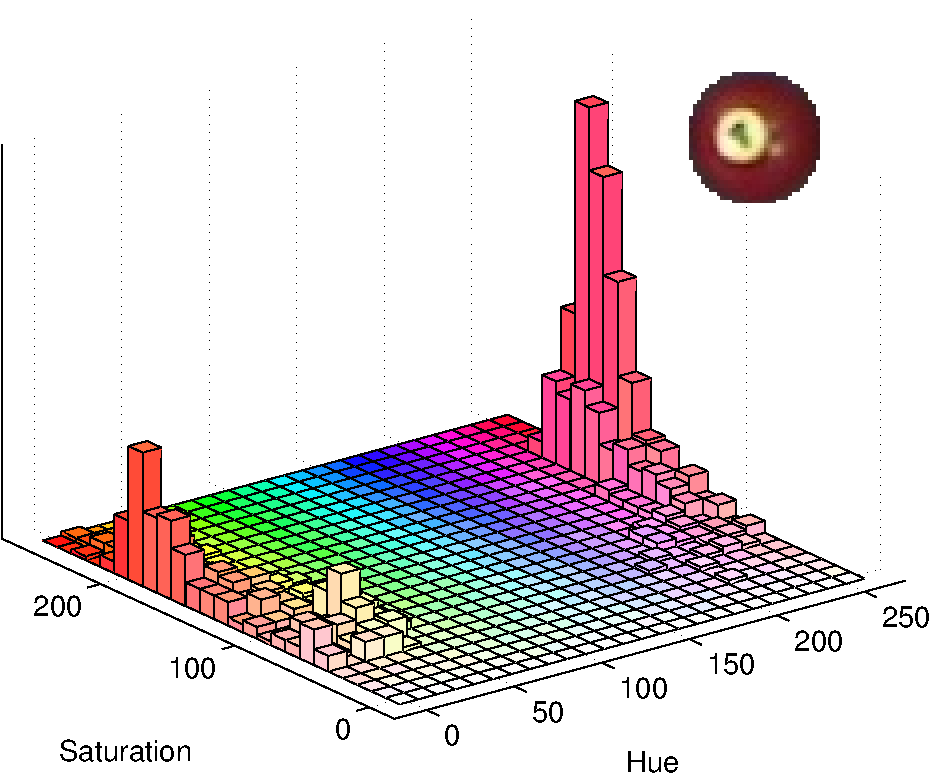
\includegraphics[width=0.4\textwidth]{images/ballhist/7}
}

\caption{Color histogram of balls: 3, 5 and 7}
\label{fig:ballhist-3-7}
\end{figure} 
Figure \ref{fig:ballhist-3-7} shows a situation where the balls are going to be difficult to separate. Depending on the lighting and camera settings, the color of 3, 5 and 7 have almost the same hue, and are only separable in saturation.

The histograms in figure \ref{fig:ballhist-3-7} also show one of the weaknesses of using HSB colorspace which is the that hue is defined an angular value that wraps between minimum and maximum. The consequence of this is that the 3 balls which has red as their dominant hue have one distribution near minimum hue and one near maximum.
\begin{figure}[H]
\centering
\subfloat
{
	
\includegraphics[width=0.4\textwidth]{images/ballhist/2}
}
\subfloat
{
	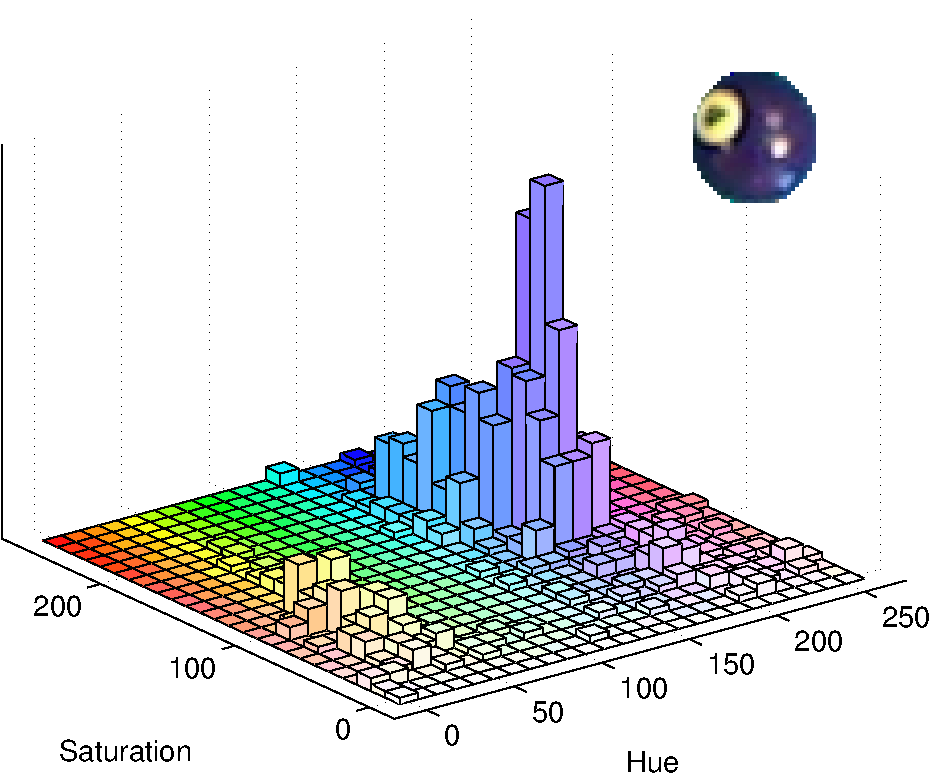
\includegraphics[width=0.4\textwidth]{images/ballhist/4}
}
\caption{Color histogram of balls: 2 and 4}
\label{fig:ballhist-2-4}
\end{figure}
Figure \ref{fig:ballhist-2-4} shows that the blue and purple balls are also challenging to separate.

\begin{figure}[H]
\centering
\subfloat
{
	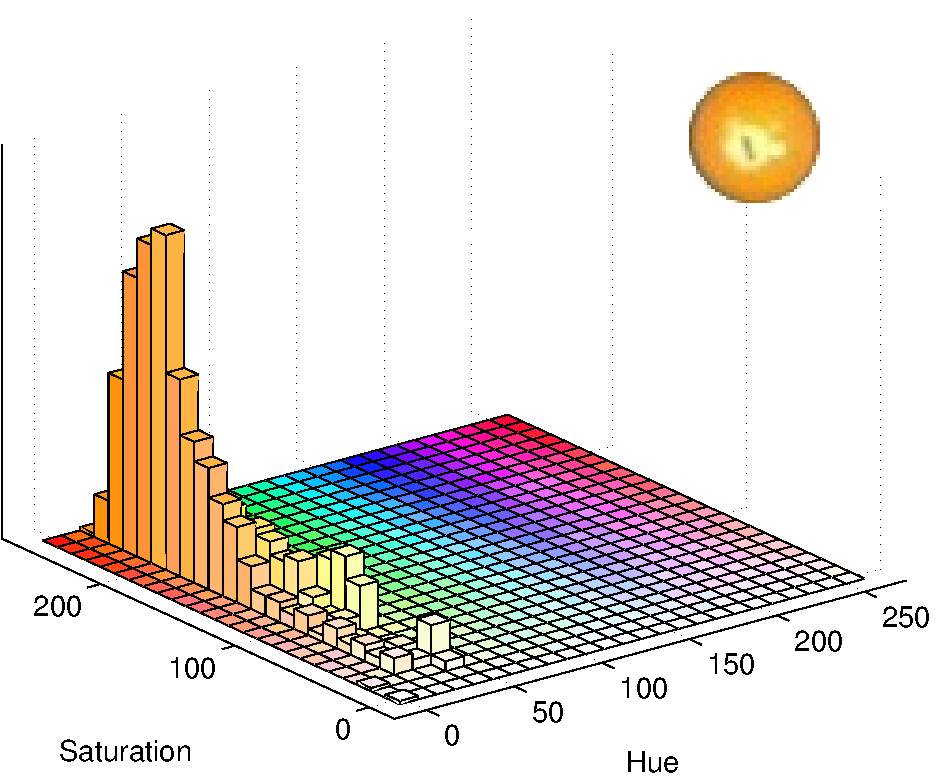
\includegraphics[width=0.4\textwidth]{images/ballhist/1}
}
\subfloat
{
	
\includegraphics[width=0.4\textwidth]{images/ballhist/6}
}
\caption{Color histogram of balls: 1 and 6}
\label{fig:ballhist-1-6}
\end{figure} 
Figure \ref{fig:ballhist-1-6} shows the two balls which do not have close neighbors. The green ball does however contain colors that are very similar to the color of the table cloth, making it harder to separate from the background than the rest.



\textbf{Ball color composition}\\
To be able to detect whether or not a ball is solid or striped it is important to know how much white is in a ball. The images used can be seen in figure \ref{fig:ballscompo} which is based on the balls used in this project.

\begin{figure}[H]
\centering
\subfloat[Solid ball with number turned up.]
{
	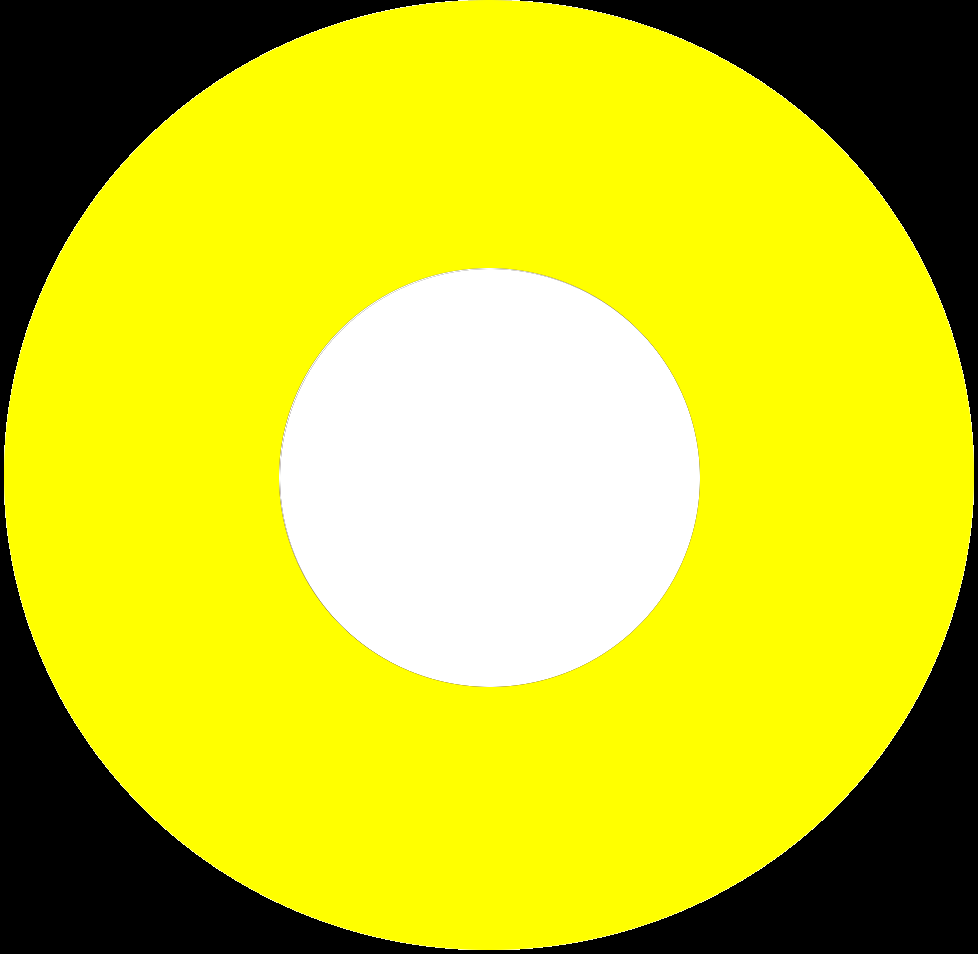
\includegraphics[width=0.2\textwidth]{images/fy.png}
}
\subfloat[Striped ball with minimum white.]
{
	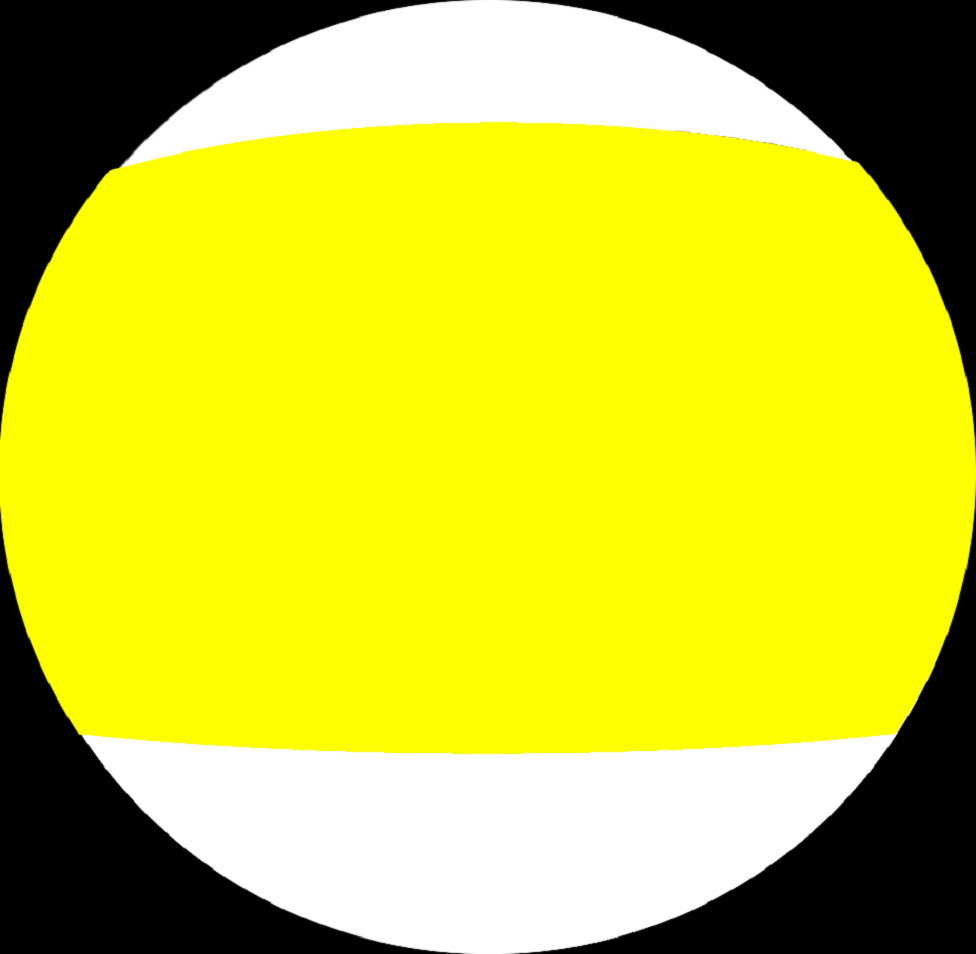
\includegraphics[width=0.2\textwidth]{images/fymax.png}
}
\subfloat[Striped ball with maximum white.]
{
	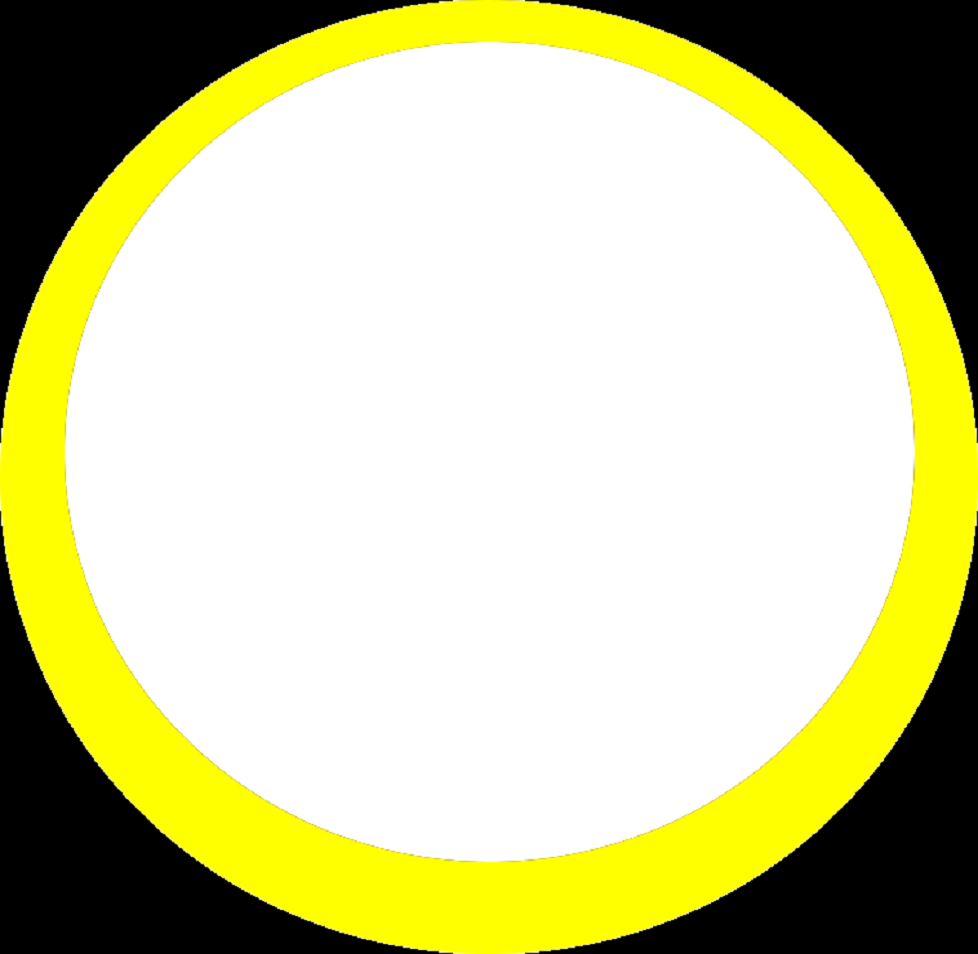
\includegraphics[width=0.2	\textwidth]{images/fymin.png}
}

\caption{Ball color compositions.}
\label{fig:ballscompo}
\end{figure}

In table \ref{fig:ballscompotable} the percentage of white pixels can be seen.\\


\begin{table}[H]
\centering
\begin{tabular}{|c|c|c|c|}
	\hline Figure & a) & b) & c) \\ 
	\hline Color & 583217 & 548839 & 175858 \\ 
	\hline White & 137359 & 173401 & 542900 \\ 
	\hline Percentage & 19.0\% & 24.0\% & 75.5\% \\ 
	\hline
\end{tabular}
\caption{Table with ball color composition.}
\label{fig:ballscompotable}
\end{table}

